\section{Theorie}
\label{sec:Theorie}
%%%%%
\subsection{Berechnung der Suszeptibilität}
\label{subsec: Berechnung}
Es gilt für die magnetische Flussdichte und Feldstärke im Vakuum
\begin{equation}
\label{eq:eq1}
\vec{B} = \mu_0 \vec{H},
\end{equation}
wobei $\mu_0$ die magnetische Feldkonstante ist. Die Flussdichte ist außerdem auch von der Magnetisierung $\vec{M}$ der sich im Feld befindenden Materialien abhängig. Die Magnetisierung
$\vec{M}$ wiederum ist auch von der magnetischen Feldstärke $\vec{H}$ abhängig. Somit gilt
\begin{equation}
\label{eq:eq2}
\vec{B} = \mu_0 \vec{H} + \vec{M}.
\end{equation}
und
\begin{equation}
\vec{M} = \mu_0 \chi \vec{H}
\end{equation}
Fügt man dies nun zusammen in \autoref{eq:eq1} ein, erhält man final
\begin{equation*}
\vec{B} = \mu_0 \vec{H} + \mu_0 \chi \vec{H},
\end{equation*}
wobei $\chi$ die Suszeptibilität beschreibt. Die Suszeptibilität ist materialabhängig, jedoch keine Konstante, da sie von der Temperatur und der Feldstärke abhängig sein kann. 
%%%%%
Das Phänomen des Paramagnetismus ist nicht bei jedem Material zu beobachten, sondern nur bei solchen, deren Drehimpuls nicht verschwinden kann.
Es entsteht in Materialien deren Atome ein magnetisches Moment zu einem äußeren Feld besitzen. Weil die Orientierung der magnetischen Momente durch die thermische Bewegung
der Atome dauerhaft geändert wird, sind die paramagnetischen Effekte temperaturabhängig.

Es soll nun der Zusammenhang zwischen dem magnetischen Moment und dem Drehimpuls betrachtet werden.
Der Gesamtdrehimpuls $\vec{J}$ setzt sich aus dem Bahndrehimpuls der Elektronenhülle $\vec{L}$, dem Spin der Elektronen $\vec{S}$ und dem Kerndrehimpuls zusammen, wobei letzterer vernachlässigt
werden kann
\begin{equation*}
\vec{J} = \vec{L} + \vec{S},
\end{equation*}
Aus der Quantenmechanik folgt:
\begin{align*}
\vec{\mu_\text{L}} &= -\frac{\mu_\text{B}}{\hbar}\vec{L} \\
\vec{\mu_\text{S}} &= -g_\text{S}\frac{\mu_\text{B}}{\hbar}\vec{S},
\end{align*}
wobei $g_\text{S}$ das gyromagnetische Verhältnis und $\mu_\text{B}$ das Bohrsche Magneton sind.

\begin{figure}[H]
	\centering
	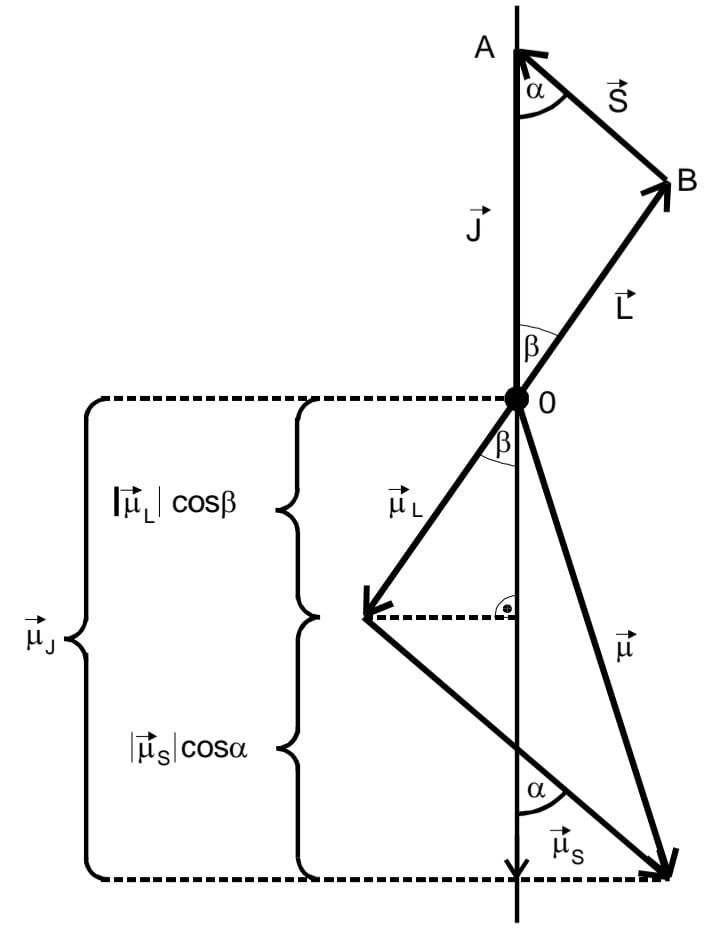
\includegraphics[width=0.6\linewidth]{data/vektordiagramm.jpeg}
	\caption{Vektordarstellung der Drehimpulse in einer Elektronenhülle und der magnetischen Momente.}
	\label{fig:vektordarstellung}
\end{figure}

Mit Hilfe der Beziehung
\begin{equation*}
\left|\vec{J}\right| = \sqrt{J(J+1)}\hbar,
\end{equation*}
die analog für $\left|\vec{L}\right|$ und $\left|\vec{S}\right|$ gilt, ergeben sich für die Beträge der magnetischen Momente die Ausdrücke
\begin{align}
\label{eq:eq3}
\left|\vec{\mu_\text{L}}\right| &= \mu_\text{B}\sqrt{L(L+1)} \\
\left|\vec{\mu_\text{S}}\right| &= g_\text{S}\mu_\text{B}\sqrt{S(S+1)}.
\end{align}
Aus diesen Beziehungen und \autoref{ABBILDUNG} ergibt sich für $\left|\vec{\mu_\text{J}}\right|$:
\begin{equation}
\left|\vec{\mu_\text{J}}\right| = \left|\vec{\mu_\text{S}}\right|\text{cos}\alpha + \left|\vec{\mu_\text{L}}\right|\text{cos}\beta.
\end{equation}
Es wird nun angenommen, dass das gyromagnetische Verhältnis den Wert $2$ annimmt. Durch diese Näherung lässt sich das magnetische Moment des Gesamtdrehimpulses zu
\begin{equation}
\label{eq:eq4}
\left|\vec{\mu_\text{J}}\right| \approx \mu_\text{B} \sqrt{J(J+1)} \frac{3J(J+1)+S(S+1)-L(L+1)}{2J(J+1)}
\end{equation}
vereinfachen. Aus dieser Gleichung wird der letzte Teilausdruck
\begin{equation*}
g_\text{J} = \frac{3J(J+1)+S(S+1)-L(L+1)}{2J(J+1)}
\end{equation*}
als Land\'{e}-Faktor zusammengefasst.

Ein weiteres relevantes Phänomen in der Quantenmechanik ist die Richtungsquantelung. Dieses besagt, dass nur Winkel zwischen der Richtung des äußeren Magnetfelds und der Lage von
$\left|\vec{\mu_\text{J}}\right|$ möglich sind, bei denen die $z$-Komponente von $\vec{\mu_\text{J}}$ in Feldrichtung ein ganzahliges Vielfaches von $\mu_\text{B}g_\text{J}$ ist.
Also gilt
\begin{equation}
\label{eq:eq5}
\mu_{\text{J}_\text{Z}} = - \mu_\text{B}g_\text{J}m,
\end{equation}
wobei $m$ die Orientierungsquantenzahl ist. Der Winkel hat somit nur $2J+1$ mögliche Einstellungsmöglichkeiten. Für jede dieser Einstellungen existiert eine potentielle Energie,
die gegeben ist als
\begin{equation*}
	\label{eq:Energie}
E_\text{m} = - \vec{\mu_\text{J}}\vec{B} = \mu_\text{B}g_\text{J}mB.
\end{equation*}

Die Aufspaltung des Energieniveaus in $2J+1$ Unterniveaus unter dem Einfluss eines äußeren Magnetfeldes wird als $\mathit{Zeeman-Effekt}$ bezeichnet.

Um nun mit Hilfe von \autoref{eq:Energie} die Magnetisierung einer Probe zu bestimmen, muss die Häufigkeit, mit der eine bestimmte Orientierung der magnetischen Momente auftritt berechnet
werden. Diese muss dann mit dem zugehörigen Betrag des Momentes nach \autoref{eq:eq5} multipliziert und anschließend über alle vorkommenden Orientierungen summiert werden:
Mit Hilfe mehrerer quantenmechanischen Betrachtungen und Nährungen lässt sich ein Ausdruck für $\chi$, das sogenannte $\mathit{Curie-Gesetz}$, herleiten.
Dieses lautet
\begin{equation}
\label{eq:mariecurie}
\chi = \frac{\mu_0\mu_\text{B}^{2}g_\text{J}^{2}NJ(J+1)}{3kT},
\end{equation}
wobei $N$ die Anzahl der Momente pro Volumeneinheit, $k$ die Boltzmann-Konstante und $T$ die Temperatur sind.
Für hinreichend hohe Temperaturen ist die Suszeptibilität $\chi$ also proportional zu $\frac{1}{T}$.

Das Phänomen des Paramagnetismus wird insbesondere bei Ionen Seltener Erden beobachtet und durch $4$f-Elektronen hervorgerufen. Daraus lässt sich schließen, dass die
inneren Elektronen große Drehimpulse besitzen müssen. Die Anordnung der Elektronen in der $4$f-Schale und der sich daraus ergebende Gesamtdrehimpuls sind in den Hundschen Regeln
festgelegt. 

1. Der Gesamtspin $\vec{S}$ nimmt den maximal möglichen Wert an, der nach dem Pauli-Prinzip zulässig ist. 

2. Die Zusammensetzung der Bahndrehimpulse $\vec{l_\text{i}}$ bildet nach $\vec{L} = \sum \vec{l_\text{i}}$ den maximalen Drehimpuls der nach Regel 1 und dem Pauli-Prinzip möglich ist.

3. Ist eine Schale höchstens zur Hälfte gefüllt, ist der Gesamtdrehimpuls $\vec{J} = \vec{L} - \vec{S}$. Bei einer mehr als zur Hälfte gefüllten gilt hingegen
$\vec{J} = \vec{L} + \vec{S}$.

\subsection{Messung der Suszeptibilität}
\begin{figure}[H]
	\centering
	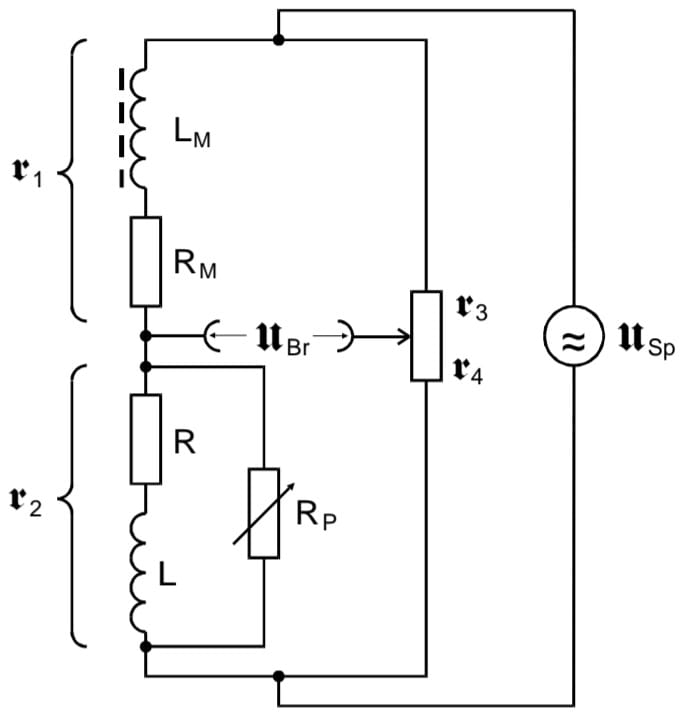
\includegraphics[width=0.7\linewidth]{data/brueckenschaltung.jpeg}
	\caption{Brückenschaltung für die Messung der Suszeptibilität.}
	\label{fig:bruckenschaltung}
\end{figure}
Für die Messung von $\chi$ wird eine Brückenschaltung wie in \autoref{fig:bruckenschaltung} mit zwei Induktivitäten verwendet. Mit Hilfe dieser Schaltung wird die
Induktivität der Spule, in der die zu untersuchende Probe liegt, gemessen.

Aus der Induktivität kann dann die Suszeptibilität $\chi$ berechnet werden.
\begin{equation}
\label{eq:indu}
L_\text{M} = \mu_0 \frac{n^2F}{l} + \chi \mu_0 \frac{n^2Q}{l}
\end{equation}
Hierbei ist $n$ die Windungszahl, $l$ die Länge, $F$ der Querschnitt der Spule und $Q$ die Querschnittfläche der Probe sind.
Der zweite Summand aus \autoref{eq:indu} ist die Induktivitätsdifferenz $\Delta L$ zwischen materiegefüllten und vakuumgefüllten Spulen.
Für die Messung der Suszeptibilität $\chi$ gibt es zwei unterschiedliche Methoden.
Bei der ersten wird die Brücke zunächst abgeglichen und anschließend eine der beiden Spulen mit dem zu untersuchenden
Material gefüllt. Die Suszeptibilität $\chi$ des Materials kann so aus der nun zu messenden Brückenspannung $U_\text{Br}$ errechnet werden.
Die Brückenspannung ist nach Kirchhoff
\begin{equation*}
U_\text{Br} = \frac{R_1R_4-R_3R_2}{(R_1+R_2)(R_3+R_4)}U_\text{Sp}.
\end{equation*}
Daraus folgt die Abgleichbedingung für die Brückenspannung
\begin{equation*}
R_1R_4 = R_3R_2.
\end{equation*}
Der Widerstand $R_1$ ist gegeben durch
\begin{equation*}
R_1 = R_\text{M} + j \omega L_\text{M}.
\end{equation*}
Mit den Näherungen $R_\text{p} \gg R $ und $R_\text{p} \gg \omega L$ ergibt sich $R_2$ zu
\begin{equation*}
R_2 \approx R + j \omega L.
\end{equation*}
Für sehr hohe Frequenzen $\omega^2 L^2 \gg R^2$ kann die Suszeptibilität vereinfacht werden zu
\begin{equation}
\chi(\omega \rightarrow \infty) = 4 \frac{F}{Q}\frac{U_\text{Br}}{U_\text{Sp}},
\end{equation}
wobei $U_\text{Sp}$ die Speisespannung ist.
Bei der zweite Methode zur Bestimmung der Suszeptibilität $\chi$ wird erneut die Brücke abgeglichen und danach eine Spule mit Material gefüllt. Anschließend wird die Brücke erneut
abgeglichen und die Suszeptibilität aus den veränderten Werten der Abgleichelemente berechnet.
Zum Abgleichen der Brücke muss also $R_3$ angepasst werden.
\begin{equation*}
R_3' = R_3 + \Delta R.
\end{equation*}
Aus den angepassten Abgleichbedingungen folgt für die Suszeptibilität $\chi$
\begin{equation}
\chi = 2 \frac{\Delta R}{R_3}\frac{F}{Q}
\end{equation}
wobei $R_3$ der Widerstand am Potentiometer ist und $\Delta R$ die Differenz zum Abgleich mit luftgefüllter Spule.

\cite{sample}
